\documentclass{article}
\usepackage[utf8]{inputenc}
\usepackage{amsmath}
\usepackage{amssymb}
\usepackage{bm}
\usepackage{color}
\usepackage{graphicx}
\usepackage{comment}
\usepackage{tikz} 
\usepackage{verbatim}
\usepackage[final]{pdfpages}

\title{IN-STK5000 Project 1 - Project 5}
\author{Anders Bredesen Hatlelid \\
        Jacob Nicolai Arthur Sjødin \\
        \and
        Even Tronstad \\
        Torgeir Ladstein Waagbø 
}

\date{\today}
\begin{document}
\maketitle


\section{Our Utility}

We define utility $U(X, Y, A)\to\mathbb{R}$ (i.e. a function of pre vaccine/treatment features, post treatment features and the action we took) as the sum of rewards for each individual. The rewards are a weighted sum of the outcomes:

$$
U(X,Y,A) = \sum_{i=1}^{N}r_i(x_i, y_i, a_i)
$$
And reward is the weighted sum of symptoms:

$$
r_i^{\text{no action}} = w^Ty
$$

$$
r_i^{a_i} = w^Ty\cdot2 - \operatorname{Cost} (a_i)
$$

(Currently we ignore the features in our utility. This implies for instance that any-one dying is equally bad, regardless of their prior condition. Which is not necceastily a good property of our utility)

We can let 'Cost' be the monetary cost of the treatment/vaccine. I.e. 100\$.

Further, we set the rewards to be all lower than zero, making it a loss function of sort, which implies that a utility of zero is the absoulte best. This makes the 'action' reward worse than the 'no action', refelcting that interfering is worse than not. If at a later stage we have more vaccines, then we must tune the coefficient more carefully.

\section{Expected utility}
For each action we can calculate the expected utility given this formula:
$$
\operatorname{E}_{a_i} U = \sum_{y\in Y}U(x, y, a_i)\cdot p(y|x, a_i)
$$
We can then choose the action $a_{best}$ which maximizes this expectation. However, since we do not know $p(y|x,a_i)$, we must estimate it with a model.
Since we assume the symptom to be independent of each other, we can simplify the expected reward $Er_i = Ew^Ty$ as the weighted sum
of expected symptoms:

\begin{equation}
    \operatorname{E}r_i = \sum_{i \in |S|} w_i\operatorname{E}(s_i)
\end{equation}



\section{Our model of choice}

We will estimate $p(s_i|a_t )$ using a beta - Bernoulli model (like in the last project), 
where we model the probability of a symptom as independently with different $\theta_i$. To update this model, we need a summary statistic, i.e. the number of sick given treatment, and the number of sick given no treatment. Since this is a simple count, it has a sensitivity of 1, making the implementation of the Laplace mechanism easy. 

For the decision of giving treatment, using a privacy method adapted for database 
squeries makes little sense, because a single decision would be equivalent with a database with one row. Therefore, we choose the randomized response mechanism, with some parameter $p$ to be decided. 

\section{Differential Privacy}
The definition of differential privacy is from the book:
Definition 3.4.2 ($\epsilon$-Differential Privacy). A stochastic algorithm $ \pi: X \to A$, where X is
endowed with a neighbourhood relation N, is said to be $\epsilon$-differentially private if:

$$
|\ln \frac{\pi(a|x)}{\pi(a|x')} | \leq \epsilon
$$

In particular: If $\pi$ is a counting algorithm, i.e.

$$
\pi(a|x) = \sum_{i} 1(x \text{ satisiying some condition})
$$
Then the centralized Laplace algorithm is $\epsilon$-differentially given $\lambda =  1/\epsilon$. This is due to the fact that a counting function has sensitivity 1, because given a database $x$ and a neighboring database $x'$ (i.e. $xNx'$ is satisfied), then the diverging row could either satisfy the same condition, making the count equal, or not satisfy the condition, making the count one less.
We therefore use the Laplace mechanism in the beta - Bernoulli model explained below:
\begin{equation}
    \begin{split}
    \theta_i \sim \operatorname{Beta}(a, b)\\
    y_i \sim \operatorname{Bernoulli}(\theta_i)\\
    \theta_i | y_i \sim \operatorname{Beta}(a', b')
\end{split}
\end{equation}


Where $a'$ and $b'$ are given by the Laplace mechanism instead of the usual counting:

\begin{equation}
    \begin{split}
        c &= \sum_{j=1}^{n} y_{i,j} + Laplace(1/\epsilon)\\
        a' &= a + c\\
        b' &= b + n - c
    \end{split}
\end{equation}


\section{Additively updating our model}
When updating our model, we have the possibility of either using the former posterior as a new prior, adding the noisy count, and proceeding as normal, however this would also add an increasing amount of Laplace noise. Another possibility is to retrain using our original prior and accumulated data. In this case, we must consider the privacy of repeated queries to our Data base. Let's say we in total apply $Q$ queries, giving the total DP of:
$$
    \sum_{i=1}^{Q} \epsilon = Q\epsilon
$$
To still achieve the same $\epsilon$-differentially privacy, we must then use $\epsilon_Q = \epsilon/Q$. This could decrease the total noise at the end of our application of the policy, however it would apply greater noise in the beginning. Since our model is the least accurate in the beginning, this in undesirable. Therefore, we choose the accumulation approach.

\section{Randomized response}
For any given individual, the decision to vaccinate is given but the maximizer of the reward, given a randomized response.
The response has the following structure:

* Flip a coin with probability $\theta_1$. If heads, answer truthfully.
* If tails, flip another coin with probability $\theta_2$ and answer yes or no given heads or tails. 

The goal of this mechanism is to satisfy the following equation:

$$
p(y|y') = \frac{p(y'|y)p(y)}{p(y')} = p(y)
$$
Where $y$ is the truth and $y'$ is the answer. In other words, knowing the response of the individual gives no additional information useful for determining the probability $y$ being true. It follows that $p(y'|y) = p(y')$ to achieve this.


\begin{equation}
    \begin{split}
        p(y'|y) &= p(\text{answer 'yes' when it is the truth})\\
 &= p_{f1} + (1-p_{f1})p_{f2} = \theta_1 + (1-\theta_1)\theta_2\\
p(y'|\overline{y}) &= (1-\theta_1)\theta_2\\
p(y') &= p(y)p(y'|y) + (1-p(y))p(y'|\overline{y})\\
&= p(y)(\theta_1 + (1-\theta_1)\theta_2) + (1-p(y))((1-\theta_1)\theta_2)
\end{split}
\end{equation}

Where $p_{fi}$ is the probability of flip number $i$ giving heads. (to be continued...)

\section{Further objectives and questions}
We did not manage in time to test the effects of privacy in this run, however we have 
made our methods flexible enough to easily add it later. We are however wondering if our results
make sense, like for instance 100\% of the population having fever, and no other symptoms.

We are also unsure if the randomized response is are favorable as opposed to the exponential method.
Since we do have a utility function, using it seems plausible, however the utility in that particular use
case is regarding the usefulness of the statistic, not the health of a population.

\section{Source code}
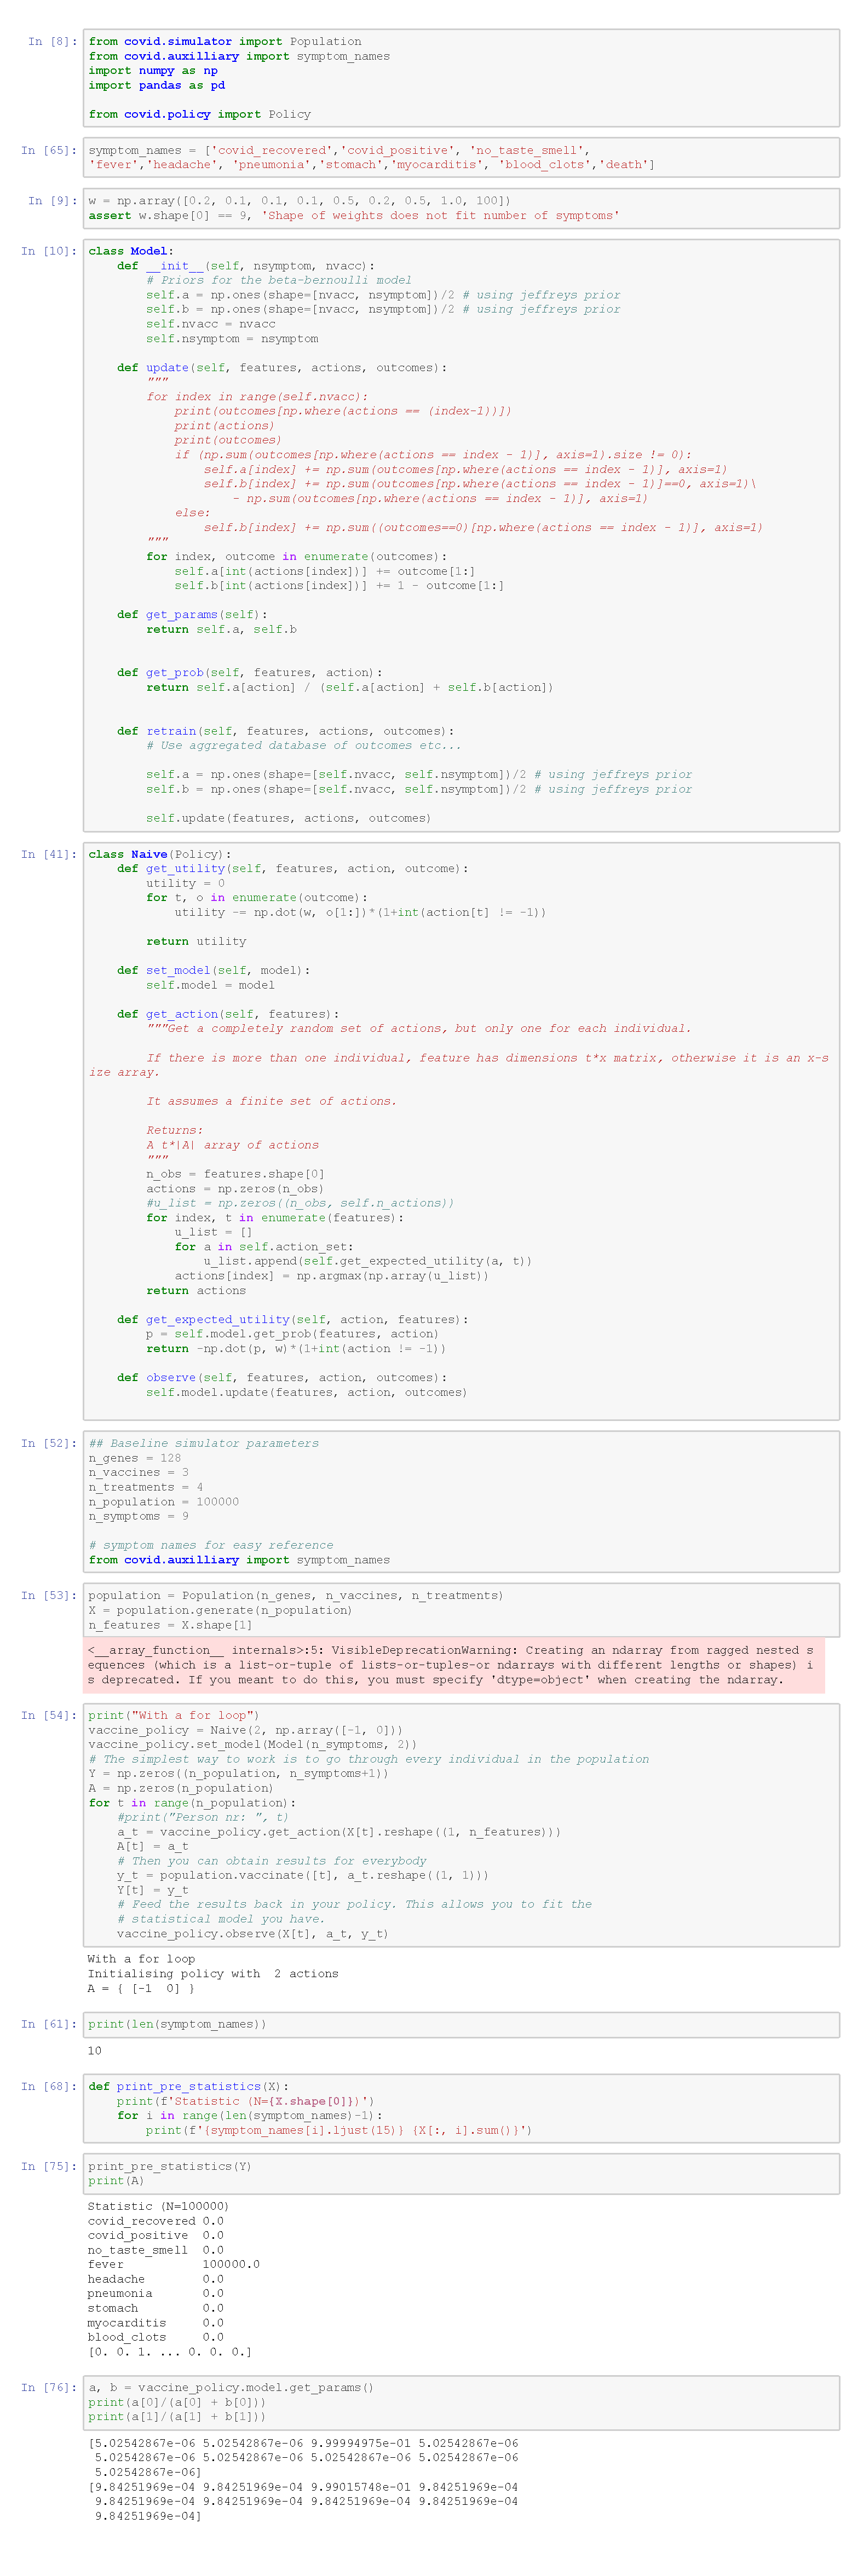
\includepdf[pages=-]{../src/policy.pdf}

\end{document}